%
\documentclass{chi-ext}
% Please be sure that you have the dependencies (i.e., additional LaTeX packages) to compile this example.
% See http://personales.upv.es/luileito/chiext/

%% EXAMPLE BEGIN -- HOW TO OVERRIDE THE DEFAULT COPYRIGHT STRIP -- (July 22, 2013 - Paul Baumann)
% \copyrightinfo{Permission to make digital or hard copies of all or part of this work for personal or classroom use is granted without fee provided that copies are not made or distributed for profit or commercial advantage and that copies bear this notice and the full citation on the first page. Copyrights for components of this work owned by others than ACM must be honored. Abstracting with credit is permitted. To copy otherwise, or republish, to post on servers or to redistribute to lists, requires prior specific permission and/or a fee. Request permissions from permissions@acm.org. \\
% {\emph{CHI'14}}, April 26--May 1, 2014, Toronto, Canada. \\
% Copyright \copyright~2014 ACM ISBN/14/04...\$15.00. \\
% DOI string from ACM form confirmation}
%% EXAMPLE END -- HOW TO OVERRIDE THE DEFAULT COPYRIGHT STRIP -- (July 22, 2013 - Paul Baumann)

\title{Firmware: The Missing Blueprint}

% Notice how author names are alternately typesetted to appear ordered in 2-column format;
% i.e., the first 4 autors on the first column and the other 4 auhors on the second column.
% Actually, it's up to you to strictly adhere to this author notation.
\author{
  \alignauthor{
        \textbf{Cefn Hoile}\\
        \affaddr{Highwire DTC}\\
        \affaddr{Lancaster University}\\
        \email{c.hoile@lancaster.ac.uk}
  }
  \vspace{2em}
  \begin{figure}
  \centering
  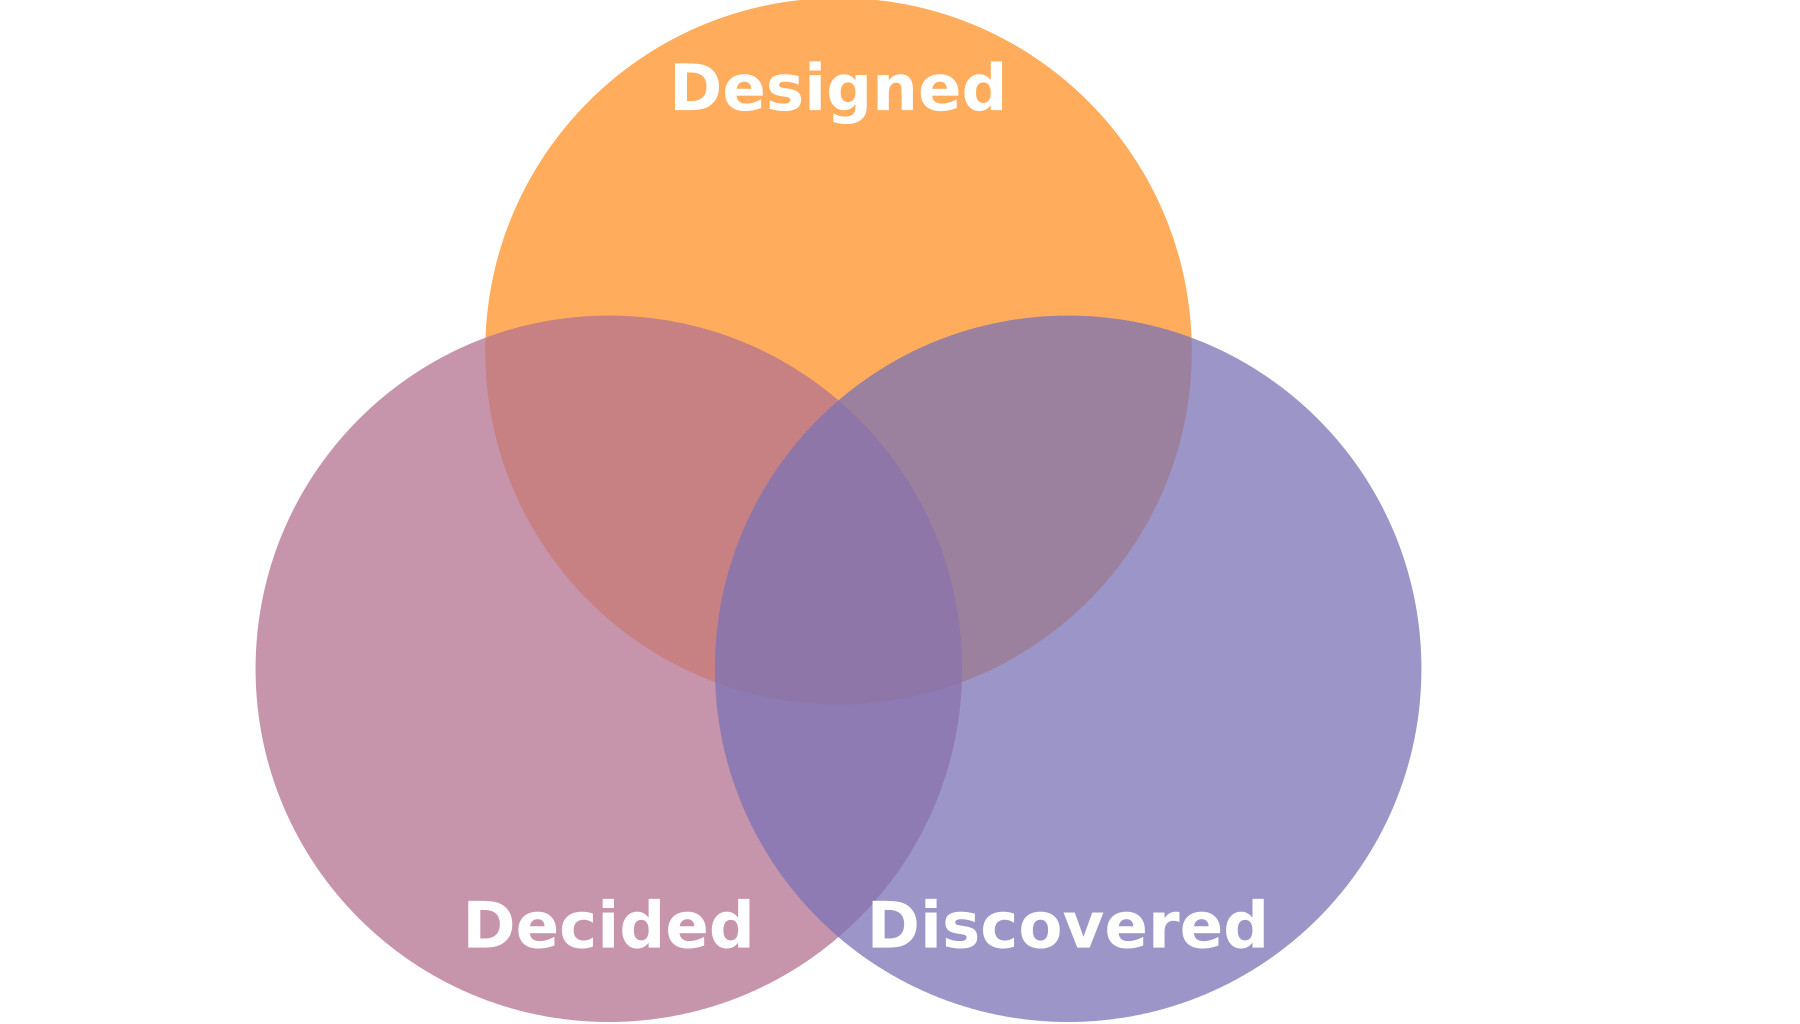
\includegraphics[width=270]{disciplines.jpg}
  \end{figure}
  \vspace{2em}
}

% Paper metadata (use plain text, for PDF inclusion and later re-using, if desired)
\def\plaintitle{CHI LaTeX Extended Abstracts Template}
\def\plainauthor{Luis A. Leiva}
\def\plainkeywords{Guides, instructions, author's kit, conference publications}
\def\plaingeneralterms{Documentation, Standardization}

\hypersetup{
  % Your metadata go here
  pdftitle={\plaintitle},
  pdfauthor={\plainauthor},  
  pdfkeywords={\plainkeywords},
  pdfsubject={\plaingeneralterms},
  % Quick access to color overriding:
  %citecolor=black,
  %linkcolor=black,
  %menucolor=black,
  %urlcolor=black,
}

\usepackage{verbatim}
\usepackage{graphicx}   % for EPS use the graphics package instead
\usepackage{balance}    % useful for balancing the last columns
\usepackage{bibspacing} % save vertical space in references
\renewcommand{\sfdefault}{phv} % Arial
\fontsize{8.5}{10}
\begin{document}

\marginpar{
\begin{figure}
  \begin{center}
  \includegraphics[width=\marginparwidth]{blueprint_long.jpg}
  \label{fig:marginparsample}
  \end{center}  
\end{figure}
}

\maketitle

\begin{abstract}
In the process of realising a product, choices must be made about its configuration. For a digitally-controlled product, its programmed behaviour, or firmware, is an element which will heavily influence user experience. We contrast three caricatures of practice in  which product configurations either \emph{discovered}, \emph{decided} or \emph{designed}, and explore the role of  reflection, sketching and boundary objects as a foundation for the practice of design. On this analysis, established practice for selecting programmed behaviour does not satisfy the criteria for being \emph{designed}. We examine what obstacles exist to applying reflective practices when selecting the \emph{behaviour} of products, and we propose a programme to identify artefacts and processes which can facilitate this work.
\end{abstract}

\keywords{Firmware, Microcontrollers, Product Design, Design Interactions, Sketching, Boundary Objects}

\category{H.5.m}{Information interfaces and presentation (e.g., HCI)}{Miscellaneous}. 
%See \cite{ACMCCS} 
See: \url{http://www.acm.org/about/class/1998/} 
for help using the ACM Classification system.
\textcolor{red}{Mandatory section to be included in your final version.}

\terms{\plaingeneralterms}
\textcolor{red}{Optional section to be included in your final version.}

\marginpar{
\begin{figure}
  \begin{center}
  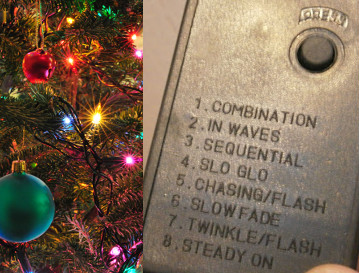
\includegraphics[width=\marginparwidth]{xmas.jpg}
  \caption{Christmas Lights}
  \label{fig:marginparsample}
  \end{center}  
\end{figure}
}

\marginpar{
\begin{figure}
  \begin{center}
  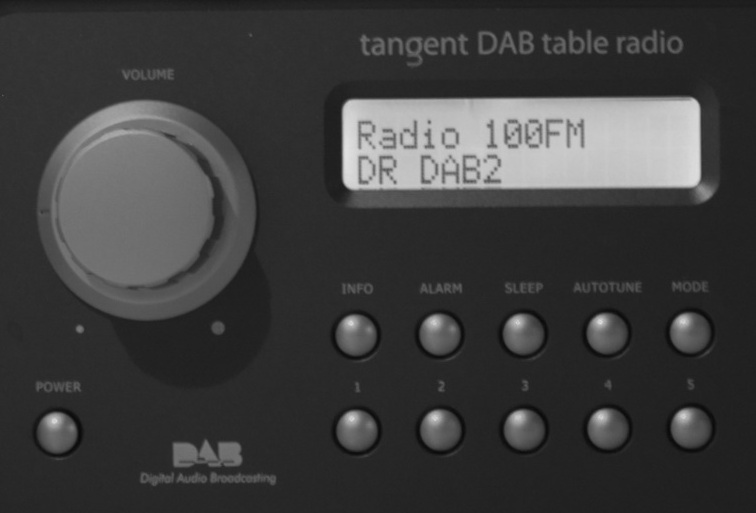
\includegraphics[width=\marginparwidth]{radio.jpg}
  \caption{Digital Radio}
  \label{fig:marginparsample}
  \end{center}  
\end{figure}
}

% =============================================================================
\section{Introduction}
% =============================================================================

An inclusive definition of design, offered by Feng and Feenberg [], is "a process of consciously shaping an artifact to adapt it to specific goals and environments". 

However, not all shaping practices adopt the same world-view. Some are close to a scientific method, where choices are \emph{discovered}, deducing them from facts. For example,  a material's physical properties can eliminate it from consideration, or experiments can recommend employing a particular approach over an alternative. Other practices map a space of solutions from which the preferred one will be \emph{decided} based on an explicit or implicit scheme of values and preferences []. 

So, is designing just discovering or decision-making? In this paper, we employ an exclusive definition of design, where the phrase \emph{designed} is reserved for preferences which are arrived at through reflective processes [Schon], where preferences are neither \emph{discovered} through evidence gathering, nor \emph{decided} through systematic analysis of a space of configurations. Instead, a designer engages in a "conversation with materials" [Schon], an operating principle captured well by Ozenc et al's [] phrase, that "the materials [designers] use begin to 'talk back'" [Ozenc et al].

Our position resonates strongly with Fallman's [], that sketching is "the archetypal activity of the design approach". However, if no candidate practices exist to parallel \emph{sketching} when selecting behaviours for a digitally controlled product, and reflective techniques are central to value-creation in all design disciplines, we may ask whether product firmware is in fact designed at all?

We characterise how sketching is employed in other design disciplines, and outline a number of reasons why these approaches cannot be trivially transferred to firmware engineering. We then propose a number of candidates for reflective materials which may be used in firmware design, and articulate the value they could bring.  


[Brock and Craft





 such as sketching 

[Brock and Craft] and bricolage [Levi-Strauss], building on design theorist's claims that  [Fallman] and that "design in all its guises is a form of bricolage"[Louridas].



Co-design or design briefing

Architecture, blueprints and patterns.

% =============================================================================
\section{Sketches and Blueprints}
% =============================================================================
Informal and formal drawings are in use throughout the design process in fashion, architecture and product design, but no analog seems to exist for interactive behaviours. Sketches and blueprints of physical designs capture implementation commitments, guiding and constraining a specialist production process. However, they also stimulate and facilitate engagement with others without demanding they themselves have the skills to materialise the design. By contrast, in a firmware design process, the3 representations which characterise implementation commitments for code are accessible principally to programmers - those skilled in materialising digital behaviours - and can not effectively catalyse knowledge exchange with others. By excluding key stakeholders until working systems are ready to be tested, this restricts the design contributions they can make, and limits the potential for design thinking. In this paper, we explore behaviour blueprints as a design fiction and a rhetorical object. We outline the preferred features by analogy with effective tools from other disciplines, and we detail a program of future co-design experimentation which we hope will allow us to explore and validate candidate representations.

\marginpar{
\begin{figure}
  \begin{center}
  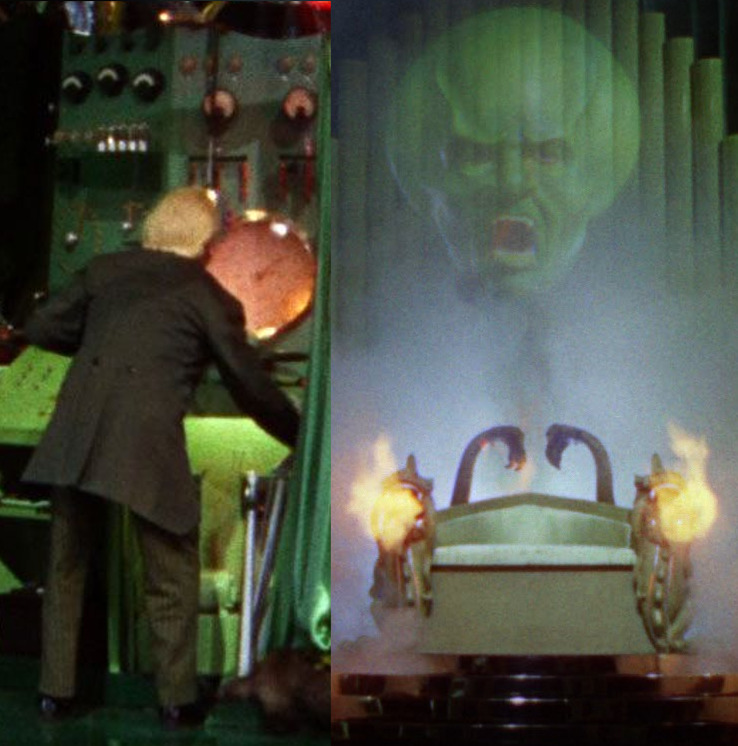
\includegraphics[width=\marginparwidth]{wizard_of_oz.jpg}
  \caption{The Wizard Of Oz}
  \label{fig:marginparsample}
  \end{center}  
\end{figure}
}

\marginpar{
\begin{figure}
  \begin{center}
  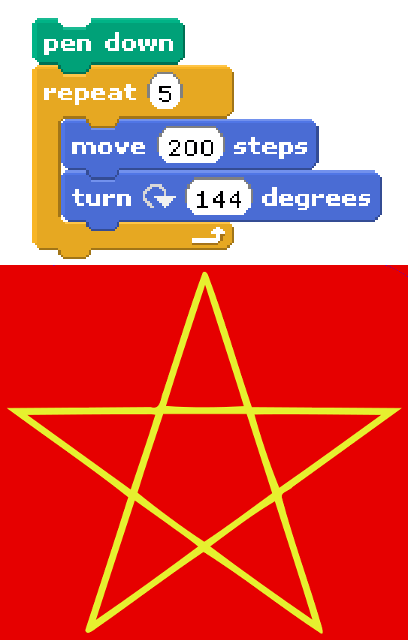
\includegraphics[width=\marginparwidth]{scratch.png}
  \caption{Scratch Programming}
  \label{fig:marginparsample}
  \end{center}  
\end{figure}
}

Van der Lugt [] observes how central ideation, reflection, storage, 

Many participants in a physical design process lack the skills needed to actually materialise the product. Nevertheless, sketches, blueprints and models can serve to catalyse knowledge exchange between a wide range of stakeholders, helping to integrate clients' experience of the market and users' experience of the domain from a very early stage in the design process of a physical product.

% =============================================================================
\section{Boundary Objects and Bricolage}
% =============================================================================
Please use an 8.5-point Verdana font, or other sans serifs font as close as possible in appearance to Verdana in {Use footnotes sparingly, if at all.}
As stated in the footnote, footnotes should rarely be used.


\begin{comment}
\begin{figure}
  \centering
  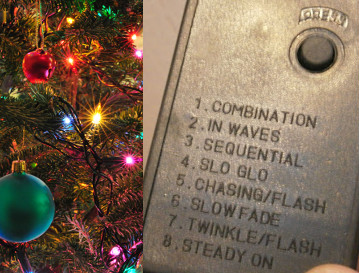
\includegraphics[width=\linewidth]{sample.jpg}
  \caption{Flashing Christmas Lights}
  \label{fig:sample}
\end{figure}
\end{comment}

% =============================================================================
\section{Conclusion}
% =============================================================================

Critiques levelled at mainstream interaction design suggest that practice should change.

\section{Acknowledgements}
NYU Dead Media Archive [Blueprint image]
Creative Commons imagery [Flickr accounts]
SarahMumOf3 for Xmas Light controller


\section{References format}
References must be the same font size as other body text.
% REFERENCES FORMAT
% References must be the same font size as other body text.

\balance
\bibliographystyle{acm-sigchi}
\bibliography{sample}

\end{document}
